% ============================================================================
% MERGED PAPER. Your Model253_Paper_With_Abstract.tex is the master for everything
% down to the References; this file is that text with four changes, each marked
% "MERGE:" so you can see and reverse any of them.
%
%  1. \affiliations{} ADDED. aaai2027.sty:132 defines \aaai@affiliations only when
%     \affiliations is called, and \maketitle (sty:169,207) uses it unconditionally,
%     so without it the build dies with "Undefined control sequence" at \maketitle.
%     Under [submission] nothing it contains is printed.
%
%  2. \clearpage REMOVED before the Appendix. The AAAI-27 kit forbids page breaks
%     of any kind; leaving it in risks a desk reject.
%
%  3. "The supplementary document" -> "Appendix E/F/G". There is no separate
%     supplementary PDF any more: that material is in this file's appendix, which
%     is excluded from the page limit, keeps the submission to one file, and lets
%     \ref{tab:main} resolve, which it cannot across two documents.
%
%  4. THREE APPENDIX SECTIONS ADDED at the end:
%       E  Evaluation conditions  (appendix_evaluation.tex, hand-written)
%       F  Additional experiments (generated from experiments.tex)
%       G  Supplementary tables   (generated from supplementary.tex)
%     F and G are produced by split_experiments.py -- run it after editing either
%     source. E is edited directly.
% ============================================================================

\pdfoutput=1
\documentclass[letterpaper]{article}
\usepackage[submission]{aaai2027}
\usepackage[hyphens]{url}
\usepackage{graphicx}
\urlstyle{rm}
\def\UrlFont{\rm}
\usepackage{natbib}
\usepackage{caption}
\usepackage{amsmath,amssymb,booktabs,array}
\frenchspacing
\pdfinfo{/TemplateVersion (2027.1)}
\setcounter{secnumdepth}{0}
\title{KAIROS: Object Discovery from Oscillatory Timing in a Spiking Network}
\author{Anonymous submission}
\affiliations{Anonymous Institution}  % MERGE 1 -- required even when anonymous
\begin{document}
\maketitle
\begin{abstract}
Can spike timing reveal which patches in a static image belong to the same object? KAIROS models image patches as coupled oscillators whose oscillatory activity controls when patches spike. We hypothesize that synchronization produces similar spike patterns in patches of the same object. KAIROS combines this similarity with image-derived connections to form object masks. It trains without ground-truth masks and infers the number of objects. Under a shared patch-level protocol, KAIROS achieves 0.841 FG-ARI on CLEVR versus 0.633 for the strongest evaluated baseline and scores higher on Tetrominoes and Multi-dSprites without additional training. On 40 held-out CLEVR images, independently shifting each patch's spike trace reduced FG-ARI from 0.865 to 0.074, indicating that our readout relies on the relative timing of activity across patches.
\end{abstract}
\section{1. Introduction}
Object-centric models such as Slot Attention bind distributed image features by assigning them to shared object representations (Locatello et al. 2020). Oscillatory models such as AKOrN add synchronization to feature processing and obtain masks by clustering the resulting representations (Miyato et al. 2025). Both leave open a complementary question: can the timing of neural activity itself tell us which regions belong to the same object?

Neurons signal through brief electrical pulses, and both how often and when they fire can matter: cortical neurons reproduce spike timings under the same fluctuating input (Mainen and Sejnowski 1995). Brain rhythms make firing more likely at some points of a cycle than others, so when two populations synchronize their windows align (Fries 2005); in cat visual cortex the strength of synchrony between sites depended on how their local stimuli formed a larger pattern (Gray et al. 1989). S$^2$-Net (Dan and Wu 2026), which our core follows, uses coupled oscillators to regulate spiking.

We hypothesize that when oscillators representing patches of the same object synchronize, their downstream neurons produce similar spike patterns.
\section{2. Method}
\begin{figure*}[t]
\centering
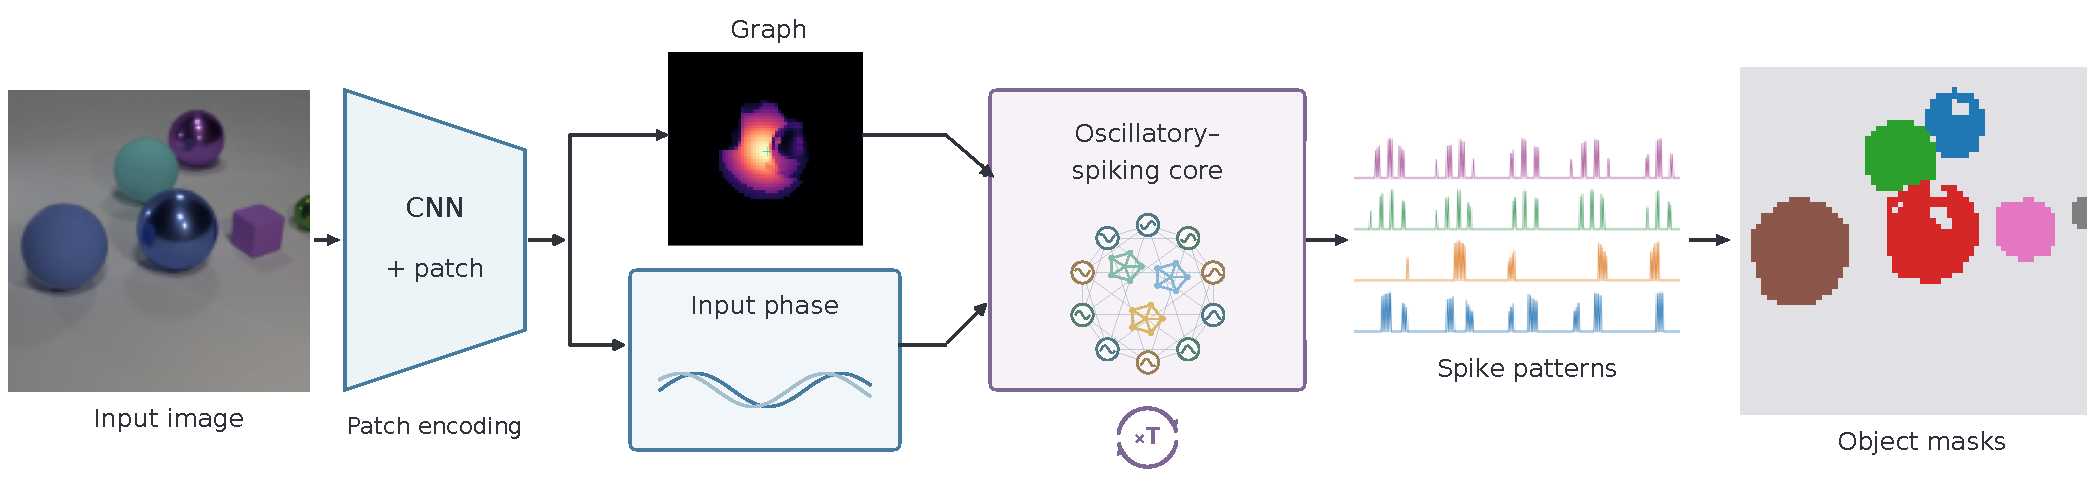
\includegraphics[width=\textwidth]{Model253_Architecture_Academic.pdf}
\caption{KAIROS overview. CNN patch features define a patch graph and input phases. The oscillatory spiking core runs for $T$ steps, and the readout combines temporal spike similarity with graph connectivity to group patches into object masks.}
\label{fig:model253}
\end{figure*}
As shown in Figure~\ref{fig:model253}, we map image patches to coupled oscillators and use their phase dynamics to modulate spiking. We then combine temporal similarity with image-derived connectivity to group patches into object masks.

\subsection{2.1 From Images to Neural Activations}
\subsubsection{2.1.1 Patch activation}
We encode an RGB image with eight convolutional filters, normalize and bound the feature maps, and pool them into a patch activation tensor $\gamma\in\mathbb R^{64\times64\times8}$. Each patch $i$ has an eight-dimensional activation vector $\gamma_i\in\mathbb R^8$. The patch indices, $i$ and $j$, identify image patches; the component index, $a$, identifies an oscillator component; and the time index, $t$, identifies a simulation step.

\subsubsection{2.1.2 Patch connection graph}
In its neuroimaging setting, S$^2$-Net (Dan and Wu 2026) uses structural connectivity to set how strongly brain regions interact. We apply the same principle to images: a weighted graph controls how strongly patch oscillators influence one another, with edge weights based on feature similarity and geodesic distance.
\begin{equation}
S_{ij}=\frac{\boldsymbol z_i^\top\boldsymbol z_j}{\tau}-r\,d(i,j).
\end{equation}
The connection score, $S_{ij}$, compares the normalized patch embeddings, $\boldsymbol z_i$ and $\boldsymbol z_j$, using the temperature, $\tau$, and penalizes the geodesic distance, $d(i,j)$, using the spatial cost weight, $r$. $\tau$ and $r$ are derived from trainable scalars.

We normalize the strongest connections and make their weights reciprocal.
\begin{equation}
\begin{gathered}
 B_{ij}=G\,\operatorname{softmax}_{j\in\mathcal N_i}(S_{ij}),\\
 A_{ij}=\frac{B_{ij}+B_{ji}}{2}.
\end{gathered}
\end{equation}
For each patch $i$, the neighbor set, $\mathcal N_i$, contains the 512 patches with the highest connection scores, $S_{ij}$. The connection gain, $G$, is derived from a trainable scalar. The normalized connection weight, $B_{ij}$, is zero for unselected neighbors. The symmetric connection weight, $A_{ij}$, defines the patch graph.

\subsubsection{2.1.3 Input phase}
We project each patch activation with the trainable weight $W_{\mathrm{drive}}$, standardize the result, and scale it with the trainable gain $W_\phi$. A scaled tanh bounds the sensory drive, $\boldsymbol\phi_i$, to $[-\pi,\pi]$. We use the bounded drive as the initial oscillator phase (Eq.~\eqref{eq:input-phase}).

\subsection{2.2 Recurrent Core}
\subsubsection{2.2.1 Kuramoto layer}
The Kuramoto layer coordinates oscillator phases across patches through intrinsic drift, patch coupling, and sensory drive. Each patch has a phase vector $\boldsymbol\theta_i(t)\in\mathbb R^4$, with one entry per oscillator.
\begin{equation}
\begin{aligned}
\boldsymbol\theta_i(t+1)={}&\boldsymbol\theta_i(t)+\Delta t\Bigl(
\boldsymbol\omega_i+f\boldsymbol\phi_i\\
&+\boldsymbol\kappa_i\odot\sin(\boldsymbol\phi_i-\boldsymbol\theta_i(t))\\
&+\frac{K}{N}\sum_j\bar A_{ij}\sin\bigl(
\boldsymbol\theta_j(t)-\boldsymbol\theta_i(t)-\alpha_{ij}\bigr)\Bigr).
\end{aligned}
\end{equation}
The \textbf{natural frequency}, $\boldsymbol\omega_i$, gives each oscillator its intrinsic rate of phase change. The \textbf{coupling term}, the sum over $j$, adjusts the phase according to other patches, using the corrected connection weight, $\bar A_{ij}$, and the phase lag, $\alpha_{ij}$. The \textbf{drive term} uses the sensory drive, $\boldsymbol\phi_i$, to adjust frequency through $f$ and to pull the phase toward the input when the drive strength, $\boldsymbol\kappa_i$, is positive. The coupling scale, $K$, is normalized by the patch count, $N$. The time step, $\Delta t$, scales the update, and $\odot$ denotes elementwise multiplication. The parameters $\boldsymbol\omega_i$, $f$, and $\boldsymbol\kappa_i$ are trainable.

\subsubsection{2.2.2 Sinusoidal gating}
The sinusoidal gating layer modulates the signal sent to the dendrites using a delayed phase. Each patch has one scalar gate $g_i(t)\in[0,1]$, shared by its four oscillator components.
\begin{equation}
\begin{gathered}
g_i(t)=\frac{1+\sin(\bar\theta_i(\max(0,t-d)))}{2}.
\end{gathered}
\end{equation}
\begin{equation}
\boldsymbol x_i(t)=g_i(t)\sin(\boldsymbol\theta_i(t)).
\end{equation}
The gate $g_i(t)$ uses the mean phase of the four oscillators (Eq.~\eqref{eq:mean-phase}) with a phase delay of $d$ steps to modulate the dendritic input $\boldsymbol x_i(t)$.

\subsubsection{2.2.3 From Gated Activity to Spikes}
Four dendritic branches integrate the current gated input with top-down feedback from the previous spike. Each branch balances its previous state with an update computed from these inputs, and the oscillatory gate modulates how much the state changes. The branch outputs are summed to drive the membrane. The membrane similarly balances its previous voltage with an update driven by the current dendritic input, with the gate modulating the size of the voltage change. When the voltage exceeds a threshold, the membrane generates a spike event, and the gate scales the emitted output. Appendix~B provides the full update equations.

\subsection{2.3 Spike Grouping and Mask Generation}
For each oscillator component, we mean-center and L2-normalize the spike trace from the last 512 simulation time steps. For patches $i$ and $j$, the correlation $\rho_{ija}$ is higher when their spike activity tends to be above or below its respective average at the same time (Eq.~\eqref{eq:spike-correlation}). We compute the patch affinity, $Q_{ij}$, by multiplying the four correlations after clipping negative values to zero. A high affinity thus requires agreement across all four components: any nonpositive correlation makes $Q_{ij}$ zero.

We form connected components by linking patch pairs with $Q_{ij}\geq0.5$ and discard components smaller than 8 patches, a floor selected on CLEVR validation. Every patch is a foreground candidate; no firing-rate test is applied. As a heuristic, we treat the largest remaining component as background, and the components that survive form the foreground support.

We start the retained foreground patches as singleton groups and merge spatially adjacent groups using
\begin{equation}
\begin{gathered}
E_{ij}=\left(1+\frac{N\bar A_{ij}}{G}\right)\log\frac{Q'_{ij}}{1-Q'_{ij}},\\
\Delta(\mathcal C,\mathcal D)=\sum_{i\in\mathcal C}\sum_{j\in\mathcal D}E_{ij}.
\end{gathered}
\end{equation}
The stabilized affinity, $Q'_{ij}$, determines the sign of the merge evidence, $E_{ij}$. The merge score, $\Delta(\mathcal C,\mathcal D)$, sums the evidence between the candidate patch groups, $\mathcal C$ and $\mathcal D$. Groups are merged while their score is positive. Each final group produces an object mask.

\section{3. Experiments}
\begin{table*}[t]
\centering
\small
\begin{tabular}{lrrrrrrrrr}
\toprule
& \multicolumn{3}{c}{CLEVR (in-domain)} & \multicolumn{3}{c}{Tetrominoes (zero-shot)} & \multicolumn{3}{c}{Multi-dSprites (zero-shot)} \\
Model & ari & f-iou & o-iou & ari & f-iou & o-iou & ari & f-iou & o-iou \\
\midrule
\textbf{KAIROS (ours)} & \textbf{.8408} & \textbf{.7528} & \textbf{.6387} & \textbf{.8568} & \textbf{.7950} & \textbf{.8170} & \textbf{.6966} & \textbf{.8190} & \textbf{.7625} \\
\midrule
AKOrN (attn) + up-tiling & .6326 & .3468 & .3636 & .5484 & .7230 & .4167 & .5505 & .6539 & .6348 \\
AKOrN (conv) & .6046 & .4219 & .2769 & .7202 & .7540 & .5913 & .4055 & .6834 & .5434 \\
AKOrN (attn) & .6027 & .3327 & .3750 & .5676 & .7383 & .4687 & .4343 & .6019 & .5751 \\
ItrSA & .5794 & .2787 & .3853 & .6319 & .7137 & .5687 & .4817 & .2489 & .6093 \\
CAE++ & .2838 & .2193 & .0882 & .2715 & .2452 & .1901 & .2648 & .1048 & .1125 \\
Slot Attention & .2872 & .2220 & .0801 & .1739 & .2192 & .1071 & .1930 & .0876 & .0680 \\
CtCAE & .2357 & .2148 & .0964 & .2681 & .2420 & .2034 & .3079 & .1158 & .1609 \\
CAE & .1091 & .2008 & .0634 & .1526 & .2305 & .1192 & .1200 & .1038 & .0630 \\
\midrule
Best baseline, per cell & .6326 & .4267 & .3853 & .7202 & .7540 & .5913 & .5505 & .6834 & .6348 \\
\textbf{Our margin} & \textbf{+.2082} & \textbf{+.3261} & \textbf{+.2534} & \textbf{+.1366} & \textbf{+.0410} & \textbf{+.2257} & \textbf{+.1461} & \textbf{+.1356} & \textbf{+.1277} \\
\bottomrule
\end{tabular}
\caption{All models trained on the same 10,000 CLEVR images for 10 epochs and evaluated on 320 held-out images per dataset by the same function; Tetrominoes and Multi-dSprites are zero-shot. Metrics are foreground ARI, foreground IoU, and matched-object IoU on the $64\times64$ patch grid. Every model uses the minimum-region-size rule of Section 3.1 at $f=0.01$. The penultimate row takes the best baseline in each cell separately, which no single baseline attains. We report one training seed. The baselines' cluster count and background mapping are selected on each target dataset's own validation split, and ours on CLEVR validation only. Appendix E states each model's conditions.}
\label{tab:main}
\end{table*}
\subsection{3.1 Protocol}
We evaluate all models with the same scoring function on a 64 \ensuremath{\times} 64 patch grid. We quantize ground-truth masks to this grid, repeat labels exactly for coarser predictions, and use patch majority voting for finer predictions. We never upsample predictions to pixels for scoring. This protocol has a score ceiling of 1.0, and its scores are not directly comparable to published pixel-level scores.

We report foreground adjusted Rand index (FG-ARI), foreground IoU (FG-IoU), and matched-object IoU (Obj-IoU) separately. Background has label 0 in both maps. FG-ARI compares partitions only on ground-truth foreground patches, so false foreground on true background does not affect it. FG-IoU compares the unions of predicted and true foreground and therefore penalizes false foreground. Appendix E gives the metric definitions.

\textbf{Training exposure.} We train every model on the same 10,000 CLEVR images for 10 epochs. For KAIROS, this corresponds to 6,250 updates with a batch size of 16, or 100,000 image exposures. We adjust only the epoch count in published baseline recipes and retain their architectures and optimizers. Table 1 evaluates transfer to Tetrominoes and Multi-dSprites without training on either dataset. Appendix E distinguishes training from validation-based tuning on the target dataset.

\textbf{Baseline readouts.} Several baselines obtain masks by clustering continuous embeddings. The reference implementations of CAE, CAE++, CtCAE, and SynCx set the cluster count to the number of unique ground-truth labels in each image. We instead use a fixed cluster count per dataset and select it and the background mapping on that dataset's validation split. This gives those baselines access to target validation data that KAIROS does not use for transfer. We make no choices on the reported split.

\textbf{Minimum region size.} Single-patch regions account for 22.8\% of KAIROS predictions on CLEVR validation, 27.0\% on Tetrominoes, and 56.2\% on Multi-dSprites. These regions arise when greedy merging splits a scattered synchronous component. They increase the predicted count with little effect on the partition. We discard regions smaller than a fraction $f$ of the image's predicted foreground. The rule uses no ground-truth labels at inference. We set $f = 0.01$ on CLEVR validation and apply it unchanged to both transfer datasets and all baselines.

\subsection{3.2 Generalization across datasets}
With matched training exposure and one training seed, KAIROS scores higher on all nine dataset--metric combinations. The reference row in Table 1 reports the best baseline for each cell, drawing from three architectures. For example, AKOrN (conv) is the closest baseline on Tetrominoes, AKOrN (attn) with up-tiling on Multi-dSprites, and ItrSA for CLEVR Obj-IoU. The smallest margin is 0.0410 for Tetrominoes FG-IoU; the other margins range from 0.128 to 0.326.

\textbf{Predicted foreground.} KAIROS predicts foreground fractions of 0.1988 on CLEVR and 0.0827 on Multi-dSprites, compared with ground-truth fractions of 0.2115 and 0.0943. On CLEVR, all baselines predict larger foreground fractions than the ground truth, ranging from 0.41 to 0.86.

\textbf{Training budget and released weights.} Slot Attention's released checkpoint, trained with roughly 320 times our exposure budget, scores lower in all nine cells by 0.377 to 0.720. Two of six baselines reach their published scores at 1/210 and 1/64 of their original schedules, respectively. For the other four, the results characterize performance at the matched training budget. Appendix F reports these comparisons, rollout lengths, and data scaling; Appendix G gives per-model results.

\subsection{3.3 Timing and object grouping}
We use the same rollouts from the first 40 held-out CLEVR images for three analyses of the hypothesis in Section 1.

\textbf{Affinity within and across objects.} We use ground-truth labels only to categorize patch pairs, without setting thresholds or object counts. The mean affinity $Q$ is 0.891 \ensuremath{\pm} 0.111 within objects, 0.047 \ensuremath{\pm} 0.048 across objects, and 0.099 \ensuremath{\pm} 0.106 between objects and background. Within-object affinity is about 19 times the across-object affinity.

\textbf{Temporal alignment.} We circularly shift each patch's four spike traces by a patch-specific offset within the readout window. This preserves each patch's firing rate and waveform while disrupting timing across patches. We keep the readout rules fixed and recompute affinities, background selection, and merges. FG-ARI falls from 0.865 to 0.074 and Obj-IoU from 0.693 to 0.033, while the mean region count rises from 7.8 to 562. FG-IoU falls from 0.803 to 0.736 because splitting a region can leave the union of predicted foreground patches nearly unchanged.

\textbf{Source of the timing signal.} The emitted spike is the product of the oscillatory gate and the binary firing indicator. The indicator is 1 in 99.99\% of settled steps, and the emitted trace correlates 0.9997 with the gate. Feeding the gate directly into the same readout reproduces every mask on all 40 images. The grouping signal therefore comes from the timing of the oscillatory gate in this experiment; we find no separate contribution from the firing threshold.

\subsection{3.4 Limitations}
\textbf{Object count.} With the minimum-size rule, KAIROS predicts 5.15 objects per image on CLEVR, 2.64 on Multi-dSprites, and 5.28 on Tetrominoes. The true means are 6.36, 2.49, and 3, and exact-count rates are 25.0\%, 53.1\%, and 9.4\%, respectively. Without the rule, predicted means rise to 8.04, 6.62, and 21.07, indicating that single-patch fragments account for much of the count error. Selecting $f$ on target validation data reduces the remaining error: on Tetrominoes, $f = 0.10$ gives a mean of 3.02 and an exact-count rate of 86.9\%. We report the transferred setting because target-specific selection uses target labels.

Tetrominoes always contains three objects. Fixed-count baselines are therefore 100\% exact even when grouping is poor (CtCAE reaches 0.0756 FG-ARI in this count comparison). On Multi-dSprites, where counts vary, these baselines are 0\% exact versus 53.1\% for KAIROS.

KAIROS trains without the reconstruction objective used by every baseline in Table 1. The absence of this penalty may help explain why KAIROS still splits some objects into parts.

\textbf{Spiking nonlinearity.} The firing indicator is saturated over the readout window (Section 3.3). The results support a role for oscillatory timing but do not isolate a contribution from thresholding. Whether sparser firing adds grouping information remains open, since the training objective does not constrain the firing rate.

\textbf{Training seeds.} We report one training seed. Reseeding one baseline changes its CLEVR FG-ARI by up to 0.134, less than the CLEVR margins in Table 1. This measures variability for that baseline and does not estimate uncertainty for KAIROS.

\textbf{Evaluation split.} The held-out images come from the training corpus, rather than an independent benchmark test set. We use published scores only for comparisons of each model with its own published results (Appendix F); Table 1 reports scores under our evaluation protocol.

\section{4. Conclusion}
KAIROS shows that an oscillatory spiking network can group image patches into object masks without mask supervision during training or a prespecified object count at inference. Under a shared evaluation protocol it reached 0.841 FG-ARI on CLEVR against 0.633 for the best evaluated baseline, and scored higher on Tetrominoes and Multi-dSprites without additional training, at a single training seed. Ablations place the grouping signal in the cross-patch alignment of the oscillatory gate rather than in the firing threshold, so the result supports relative oscillatory timing as a cue for object discovery. The rollout is costly, counting is weaker than grouping, and whether the gated traces also support object tracking is left to future work.\label{pg:body-end}

% page-budget probes: pg:body-end must resolve to page 4 or lower (4-page main text).
%   grep 'newlabel{pg:' main_full.aux   after a build.
\section*{References}\label{pg:references}
Dan, T.; and Wu, G. 2026. From Cortical Synchronous Rhythm to Brain Inspired Learning Mechanism: An Oscillatory Spiking Neural Network with Time-Delayed Coordination. arXiv:2605.01656.

Fries, P. 2005. A mechanism for cognitive dynamics: neuronal communication through neuronal coherence. \textit{Trends in Cognitive Sciences}, 9(10): 474--480.

Gray, C. M.; K\"onig, P.; Engel, A. K.; and Singer, W. 1989. Oscillatory responses in cat visual cortex exhibit inter-columnar synchronization which reflects global stimulus properties. \textit{Nature}, 338: 334--337.

Locatello, F.; Weissenborn, D.; Unterthiner, T.; Mahendran, A.; Heigold, G.; Uszkoreit, J.; Dosovitskiy, A.; and Kipf, T. 2020. Object-Centric Learning with Slot Attention. In \textit{Advances in Neural Information Processing Systems}.

Mainen, Z. F.; and Sejnowski, T. J. 1995. Reliability of spike timing in neocortical neurons. \textit{Science}, 268(5216): 1503--1506.

Miyato, T.; L\"owe, S.; Geiger, A.; and Welling, M. 2025. Artificial Kuramoto Oscillatory Neurons. In \textit{International Conference on Learning Representations}.

% MERGE 2: \clearpage removed here -- the kit forbids page breaks of any kind.
\section{Appendix}
\setcounter{equation}{0}
\renewcommand{\theequation}{A\arabic{equation}}

\subsection{A Sensory Representation and Graph Details}
The input is a $128\times128$ RGB image scaled by $\frac{1}{255}$. A single $3\times3$ convolution with eight trainable filters, unit stride, and no padding produces $126\times126\times8$ feature maps. There is no post-convolution activation. All eight channels share a scalar mean $\mu$ and standard deviation $\sigma$, estimated once from the initial encoder on training RGB images. We use $\sigma=\sqrt{\max(\operatorname{Var}(F),10^{-8})}$, where $F$ pools feature values over training images, channels, and spatial positions. We standardize with these fixed statistics and clip the result to $[-3,3]$. Adaptive average pooling produces a $64\times64$ grid, yielding $N=4096$ patch vectors with eight features each.

The bias-free trainable projection $W$ gives the embedding
\begin{equation}
\boldsymbol z_i=\frac{W\gamma_i}{\max(\lVert W\gamma_i\rVert_2,\varepsilon)}.
\end{equation}
For grid coordinates $p_i$, the scaled spatial distance and local traversal cost are
\begin{equation}
\begin{aligned}
d_{\mathrm{sp}}(i,j)&=\frac{\lVert p_i-p_j\rVert_2}{4},\\
c_{ij}&=d_{\mathrm{sp}}(i,j)[1+8(1-\boldsymbol z_i^\top\boldsymbol z_j)^2].
\end{aligned}
\end{equation}
Set $d_{ij}^{(0)}=c_{ij}$ when $d_{\mathrm{sp}}(i,j)\le1.5$ and 16 otherwise. With $\tau_{\mathrm{geo}}=0.5$, three updates ($m=0,1,2$) give
\begin{equation}
\begin{aligned}
u_{ij}^{(m)}&=-\tau_{\mathrm{geo}}\log\sum_k\exp\left(-\frac{d_{ik}^{(m)}+d_{kj}^{(m)}}{\tau_{\mathrm{geo}}}\right)\\
&\quad+\tau_{\mathrm{geo}}\log4,\\
d_{ij}^{(m+1)}&=\min(d_{ij}^{(m)},u_{ij}^{(m)}),\\
d(i,j)&=\min(d_{ij}^{(3)},16).
\end{aligned}
\end{equation}
With learned scalars $\ell_\tau,\ell_G,\ell_r$, the graph parameters are
\begin{equation}
\begin{aligned}
\tau&=\max(\exp(\ell_\tau),0.001),\qquad G=\exp(\ell_G),\\
r&=\operatorname{softplus}(\ell_r)=\log(1+\exp(\ell_r)).
\end{aligned}
\end{equation}
Each patch selects its 512 highest-scoring connections before normalization. Symmetrization can increase its degree beyond 512.

The trainable projection, $W_{\mathrm{drive}}$, maps eight features to four components without bias. Its output is standardized over all $4N$ patch-component entries of the current image with a standard deviation floor of $10^{-6}$. The trainable scalar, $W_\phi$, scales this input before tanh bounds the drive between $-\pi$ and $\pi$. The drive and graph remain fixed during a rollout. The input phase is computed as
\begin{equation}\label{eq:input-phase}
\begin{gathered}
\boldsymbol u_i=W_{\mathrm{drive}}\gamma_i,\\
\boldsymbol\phi_i=\pi\tanh(W_\phi\,\bar{\boldsymbol u}_i),\qquad
\boldsymbol\theta_i(0)=\boldsymbol\phi_i.
\end{gathered}
\end{equation}

\subsection{B Recurrent Dynamics}
\subsubsection{B1 Coupling Correction and Phase Lag}
The corrected graph stabilizes inverse connection costs and gives zero graph entries a small residual weight:
\begin{equation}
\begin{gathered}
\bar A=\operatorname{ReLU}\left(\frac{A+A^\top}{2}\right)+10^{-6},\\
C_{ij}=\frac{1}{\bar A_{ij}}.
\end{gathered}
\end{equation}
\begin{equation}
\begin{gathered}
\bar C_{ij}=\frac{C_{ij}-\min C}{\max C-\min C+10^{-6}},\\
\alpha_{ij}=\tanh(R_{ij}-R_{ji})\bar C_{ij}.
\end{gathered}
\end{equation}
The inverse connection cost, $C_{ij}$, is normalized over all patch pairs to obtain $\bar C_{ij}$. The trainable directional matrix, $R$, determines the direction of the phase lag, $\alpha_{ij}$, through its antisymmetric difference. The inverse cost sets the lag scale. This permits coordinated phases with nonzero offsets. The lag is shared by all four components.

The natural frequency, $\boldsymbol\omega_i$, controls intrinsic angular drift. The drive adjusts frequency through $f\boldsymbol\phi_i$ and provides sine forcing toward $\boldsymbol\phi_i$ when the drive strength, $\boldsymbol\kappa_i$, is positive. Coupling, drive, and drift act together; phase is not required to converge to the input phase. The coupling scale, $K$, equals $N$, and the time step, $\Delta t$, is 0.1.

\subsubsection{B2 Rhythmic Gating and Branch Integration}
We set the phase delay to $d=2$ simulation steps. The scalar gate, $g_i(t)$, is shared across the patch's four components and has no trainable parameters.

The mean patch phase averages the four component phases:
\begin{equation}\label{eq:mean-phase}
\bar\theta_i(t)=\frac{1}{4}\sum_{a=1}^4\theta_{ia}(t).
\end{equation}

The branch input combines the gated feature, $x_{ia}(t)$, with the previous emitted spike, $s_{ia}(t-1)$, through the trainable projection, $U\in\mathbb R^{4\times2}$, and the trainable bias, $\boldsymbol b\in\mathbb R^4$:
\begin{equation}\label{eq:branch-input}
\boldsymbol v_{ia}(t)=U\begin{pmatrix}x_{ia}(t)\\s_{ia}(t-1)\end{pmatrix}+\boldsymbol b.
\end{equation}
The previous spike is the top-down feedback from the spiking output to the dendritic branches.

Each branch state vector has four entries. The retention vector, $\boldsymbol\beta_i$, is obtained by applying sigmoid to the trainable retention vector, $\boldsymbol k_i$. The provisional branch state is
\begin{equation}\label{eq:branch-provisional}
\begin{aligned}
\widehat{\boldsymbol h}_{ia}(t)={}&\boldsymbol\beta_i\odot\boldsymbol h_{ia}(t-1)\\
&+(1-\boldsymbol\beta_i)\odot\boldsymbol v_{ia}(t).
\end{aligned}
\end{equation}
The gate and the trainable modulation weight, $\eta_a$, set how much of the increment toward the provisional state is applied, and summing the four entries gives the membrane input, $H_{ia}(t)$, where $b$ indexes an entry of $\boldsymbol h_{ia}(t)$:
\begin{equation}\label{eq:branch-update}
\begin{aligned}
\boldsymbol h_{ia}(t)={}&\boldsymbol h_{ia}(t-1)
+\bigl(1-\eta_a(1-g_i(t))\bigr)\\
&\quad{}\cdot\bigl(\widehat{\boldsymbol h}_{ia}(t)-\boldsymbol h_{ia}(t-1)\bigr),\\
H_{ia}(t)={}&\sum_{b=1}^{4}h_{iab}(t).
\end{aligned}
\end{equation}
Retention is shared across oscillator components of the same patch, while their branch states remain separate. Modulating the full increment also controls leakage and spike recurrence, which would continue if only the current input were gated. Summing the four entries combines branch responses without averaging oscillator components.

\subsubsection{B3 Membrane Update and Spike Emission}
The provisional membrane voltage is
\begin{equation}\label{eq:membrane-provisional}
\begin{aligned}
\widehat V_{ia}(t)={}&\lambda_iV_{ia}(t-1)+(1-\lambda_i)H_{ia}(t)\\
&-\vartheta_a s_{ia}(t-1).
\end{aligned}
\end{equation}
The membrane retention, $\lambda_i$, is the sigmoid of the trainable patch parameter, $\ell_i$. The firing threshold, $\vartheta_a$, is 0.06 times the exponential of the trainable component parameter, $q_a$. Membrane resistance is fixed to one. The subtractive reset is proportional to the previous emitted spike and does not force voltage to zero.

As in the branch update, the gate and the trainable modulation weight, $\xi_a$, set how much of the increment toward the provisional voltage is applied, and the thresholded voltage is gated to give the emitted spike:
\begin{equation}\label{eq:membrane-update}
\begin{aligned}
V_{ia}(t)={}&V_{ia}(t-1)+\bigl(1-\xi_a(1-g_i(t))\bigr)\\
&\quad{}\cdot\bigl(\widehat V_{ia}(t)-V_{ia}(t-1)\bigr).
\end{aligned}
\end{equation}
\begin{equation}\label{eq:spike-emission}
\begin{gathered}
e_{ia}(t)=\operatorname{ind}(V_{ia}(t)>\vartheta_a),\\
s_{ia}(t)=g_i(t)e_{ia}(t),
\end{gathered}
\end{equation}
where $\operatorname{ind}$ is the indicator function and $e_{ia}(t)$ is the binary firing event.

When the gate is exactly zero, the previous voltage is retained. Otherwise, the gated update is applied before thresholding. The emitted spike, $s_{ia}(t)$, enters the next branch input and membrane reset. Dendritic and membrane states and the previous spike start at zero. The rollout uses 1024 steps.

\subsection{C Temporal Affinity and Object Masks}
We retain steps $\mathcal T=\{512,\ldots,1023\}$ and index them by $m=1,\ldots,512$. Centering and L2 normalization give
\begin{equation}
\begin{aligned}
\mu_{ia}&=\frac{1}{512}\sum_{t\in\mathcal T}s_{ia}(t),\\
r_{ia,m}&=\frac{s_{ia}(511+m)-\mu_{ia}}{\max\left(\sqrt{\sum_{t\in\mathcal T}(s_{ia}(t)-\mu_{ia})^2},10^{-8}\right)}.
\end{aligned}
\end{equation}
A constant trace becomes zero. The component correlation and patch affinity are
\begin{equation}\label{eq:spike-correlation}
\rho_{ija}=\operatorname{clip}\left(
  \sum_{m=1}^{512} r_{ia,m}\,r_{ja,m},-1,1\right),
\end{equation}

\begin{equation}
Q_{ij}=\prod_{a=1}^{4}\max(\rho_{ija},0).
\end{equation}
Centering removes the baseline and normalization reduces sensitivity to absolute scale. The product requires positive temporal agreement in every component; one nonpositive correlation makes the affinity zero. The affinity is not a calibrated same-object probability.

Connected components of $Q\geq0.5$ determine the initial support without a spatial adjacency constraint. Components smaller than 8 patches are discarded, a floor selected on CLEVR validation, and the largest remaining component is treated as background. Every patch enters this step as a candidate; no activity or firing-rate threshold is applied, so the foreground is defined entirely by the synchrony structure. Removed patches are not recovered. The retained support is reset to singleton patches before merging.

The stabilized affinity is
\begin{equation}
Q'=\operatorname{clip}\left(\frac{Q+Q^\top}{2},10^{-6},1-10^{-6}\right).
\end{equation} The merge evidence, $E$, is symmetrized and its diagonal set to zero. The log-odds term gives positive evidence above 0.5 and negative evidence below 0.5. Graph weights change its magnitude without changing its sign. Merge scores sum all cross-group pairs. Only groups adjacent on the four-neighbor grid are candidates. The largest positive candidate is merged until none remains.

The hard label, $y_i$, identifies the final foreground group or equals zero for excluded patches. The binary object mask, $M_k$, selects the patches assigned to group $k$ on the $64\times64$ grid. The 8-patch floor is not reapplied after merging. If no foreground survives, the output is all background.

\subsection{D Training Details}
\subsubsection{D1 Initialization and optimization}
We train the Native64 encoder and recurrent core jointly from random initialization without loading a pretrained checkpoint. The shared dendritic bias starts at zero. Training uses RGB images without segmentation masks, object counts, or reconstruction targets.

We compute the objective separately for each image and average the resulting losses across images. After accumulating gradients, we clip the global $\ell_2$ norm across trainable parameters to 1 and apply Adam. The encoder and the other active parameter groups use separate fixed learning rates. The legacy geodesic contrast parameter is excluded from optimization because the forward operator uses a fixed contrast.

\subsubsection{D2 Rollout and gradient window}
We simulate 1,024 steps per image. Both losses use steps 512--1023 (zero-based), but recurrent backpropagation covers only steps 960--1023. The first 960 steps run without gradient tracking, and the recurrent states are detached at the boundary. The earlier steps in the loss window still contribute to the statistics. The image graph, sensory drive, and factorized coupling are computed with gradients enabled and reused in the final 64 steps, so the loss can reach the encoder through the graph and drive. The phase loss propagates through the Kuramoto dynamics, while the spike loss also trains the dendritic and membrane parameters through the emitted spike traces. A multi-Gaussian surrogate derivative supports backpropagation through the binary spike threshold. Connected-component filtering and greedy merging are used for inference and do not enter the training objective.

\subsubsection{D3 Phase and spike statistics}
The phase loss uses a phase-locking value (PLV) matrix $P$. Using the arithmetic mean phase $\bar\theta_i(t)$ from Eq.~\eqref{eq:mean-phase}, define $\delta_{ij}(t)=\bar\theta_i(t)-\bar\theta_j(t)$ and let $\langle\cdot\rangle_t$ denote the mean over steps 512--1023. Then
\begin{equation}
\begin{aligned}
R_{ij}^{\mathrm{plv}}&=\langle\cos\delta_{ij}(t)\rangle_t,\qquad
I_{ij}^{\mathrm{plv}}=\langle\sin\delta_{ij}(t)\rangle_t,\\
P_{ij}&=\operatorname{clip}\left(
\sqrt{(R_{ij}^{\mathrm{plv}})^2+(I_{ij}^{\mathrm{plv}})^2+10^{-12}},
0,1\right).
\end{aligned}
\end{equation}
A high PLV reflects a stable phase difference, which need not be zero. The spike loss uses the affinity matrix $Q$ from Appendix C, computed from the emitted, gated spikes over the same window. Unlike $P$, $Q$ multiplies the nonnegative correlations of four separate spike traces.

\subsubsection{D4 Loss function}
For $X\in\{P,Q\}$, let $\langle\cdot\rangle_{\ne}$ be the mean over all $N(N-1)$ ordered off-diagonal pairs. We use the same criterion for both matrices:
\begin{equation}
\begin{aligned}
\mathcal C(X)={}&6L_{\mathrm{bim}}(X)+10L_{\mathrm{bal}}(X)\\
&+0.5L_{\mathrm{coh}}(X)+L_{\mathrm{col}}(X),\\
L={}&\mathcal C(P)+5\mathcal C(Q).
\end{aligned}
\end{equation}
Let $\mu_X=\langle X_{ij}\rangle_{\ne}$ and $v_X=\langle(X_{ij}-\mu_X)^2\rangle_{\ne}$. The bimodality, balance, and collapse terms are
\begin{equation}
\begin{aligned}
L_{\mathrm{bim}}(X)&=\langle X_{ij}(1-X_{ij})\rangle_{\ne},\\
L_{\mathrm{bal}}(X)&=(\mu_X-0.867)^2,\\
L_{\mathrm{col}}(X)&=-\log(v_X+10^{-4}).
\end{aligned}
\end{equation}
The first favors affinities near zero or one; the second targets a fixed mean affinity of 0.867; the third penalizes low off-diagonal variance. The target is a pairwise affinity prior, not a target for object count or foreground area. The logarithmic penalty is finite at zero variance.

For spatial coherence, we reshape the off-diagonal row means $a_i=(N-1)^{-1}\sum_{j\ne i}X_{ij}$ into a $64\times64$ field $a_{r,c}$ and use
\begin{equation}
\begin{aligned}
L_{\mathrm{coh}}(X)={}&
\operatorname{mean}_{r,c}|a_{r+1,c}-a_{r,c}|\\
&+\operatorname{mean}_{r,c}|a_{r,c+1}-a_{r,c}|.
\end{aligned}
\end{equation}
Each mean includes only valid adjacent pairs in its direction. This term smooths each patch's mean affinity to the other patches; it does not operate on the final masks.

% MERGE 4: Appendices E (evaluation conditions), F (additional experiments) and
% G (per-model tables). F and G are generated by split_experiments.py.
% Appendix E -- evaluation conditions. Hand-written; not generated.
%
% Everything here is read off the implementation, not recalled:
%   patch_fg_ari            collaborative_test/evaluation.py:114
%   patch_foreground_iou    collaborative_test/evaluation.py:145
%   patch_matched_object_iou collaborative_test/evaluation.py:160
% The per-model tuning splits are read from the baselines' own *_bg.json records,
% which store the selected background rule together with the validation split and
% the image count it was selected on.

\subsection{E Evaluation Conditions}

\subsubsection{E1 What each metric can and cannot see}
All three metrics take two aligned integer label maps on the $64\times64$ patch grid, with
background as label $0$ on both sides. They differ in which patches they look at, and the
difference decides which errors are charged.

\textbf{Foreground ARI} restricts both label maps to the patches whose \emph{ground truth} is
foreground, and computes the adjusted Rand index of the two partitions of that set. Predicted
background is kept as an ordinary cluster inside it, so predicting background on a true object
is charged; but patches whose ground truth is background are removed before scoring, so
\emph{labelling background as object is invisible to this metric}. An image with fewer than two
true foreground patches is undefined and excluded; a degenerate pair of identical partitions
scores $1$.

\textbf{Foreground IoU} merges every non-background identity on each side into one set and
reports $|{\hat F}\cap F|/|{\hat F}\cup F|$ over patches. False foreground enters the union and
nothing else, so this is the metric that charges for claiming background as object --- the error
FG-ARI cannot see. Both sets empty scores $1$; exactly one empty scores $0$. This is why
Table~\ref{tab:main} is read with the two together: a method that labels most of the image as
object can hold a respectable FG-ARI while its foreground IoU collapses, which is what the
\textsc{f-iou} column shows for the baselines that predict $0.41$ to $0.86$ foreground against a
truth of $0.2115$.

\textbf{Matched-object IoU} solves a one-to-one Hungarian assignment between predicted and true
objects maximising total IoU, sums the matched IoUs and divides by the number of \emph{true}
objects, so an unmatched true object contributes zero. Background is not matched. False
foreground enlarges the unions of the objects it touches, but \emph{extra predicted objects carry
no direct penalty} beyond going unmatched. Over-segmentation is therefore not charged by this
metric, which is the reason object count is reported separately in Section 3.3 rather than
treated as covered by it. No true objects gives an undefined score; predictions empty against a
non-empty truth gives $0$.

Undefined images are excluded per metric and the remainder averaged, so the three metrics can
rest on slightly different image counts; the counts are recorded with every result. No weighted
combination of the three is formed anywhere.

\subsubsection{E2 Which split fixed each free choice}
Every method has choices that are not learned by its training objective, and a transfer claim is
only as strong as the data used to fix them. \emph{Not trained on the target} and \emph{not tuned
on the target} are different statements, and they do not hold equally for every row of
Table~\ref{tab:main}.

\textbf{Ours.} One free scalar: the minimum-region-size fraction $f$. It is fixed at $0.01$ on the
\emph{CLEVR} validation split and applied unchanged to Tetrominoes and Multi-dSprites. No
Tetrominoes or Multi-dSprites data, labelled or unlabelled, enters any choice we make. Everything
else in the readout --- the $Q\ge0.5$ link threshold, the 8-patch component floor (itself
selected on CLEVR validation), the largest-component background heuristic, the rollout length
and the readout window --- is fixed before these datasets are touched and is identical across
all three.

\textbf{Baselines.} Two free choices, and \emph{both are fixed on the target dataset's own
validation split}: the number of clusters $k$ and the rule mapping one cluster to background.
The background rule is selected from four candidates (global-largest, image-largest,
border-largest, border-union) by validation FG-ARI with foreground IoU as tie-break, separately
for each model and each dataset. For the CAE family $k$ is likewise selected per dataset from
$\{4,7,11\}$, and the selection does not land on the same value everywhere: CAE\texttt{++} uses
$k=11$ on CLEVR and Tetrominoes but $k=7$ on Multi-dSprites, and CAE uses $11$, $11$ and $4$. For
AKOrN, ItrSA and Slot Attention the slot count is the architecture's own and is left at the
authors' value, but the background rule is still chosen on the target's validation split. The
selection used $320$ validation images on CLEVR, and $1{,}000$ on Tetrominoes and Multi-dSprites
for the AKOrN family, $320$ for the CAE family.

The asymmetry runs in the baselines' favour, not ours: on the two transfer datasets they are
allowed to see target labels to set $k$ and the background mapping, and we are not. We state it
here rather than leaving "zero-shot" to carry both meanings at once. Removing the oracle that the
reference implementations of CAE, CAE\texttt{++}, CtCAE and SynCx use --- setting $k_i$ from the
per-image ground-truth object count --- is a separate and stricter correction, described in
Section 3.1; a per-dataset constant chosen on validation is what replaces it.

The minimum-region-size rule is offered to every model on the same terms, and it is not a private
advantage: applied at $f=0.01$ it leaves every baseline row of Table~\ref{tab:main} unchanged to
three decimals except AKOrN (conv) on CLEVR foreground IoU, which improves from $.4219$ to
$.4267$; the best-baseline row uses the better of the two for every baseline cell we measured.

No hyperparameter, threshold or rule of any model is selected on the $320$ reserved images that
Table~\ref{tab:main} reports. Those images are read once, after every choice is frozen.

% GENERATED by split_experiments.py from experiments.tex and supplementary.tex --
% do not edit directly. Appendix F is the two Experiments subsections that do not fit
% the four-page main text; Appendix G is the per-model tables.
%
\subsection{F Additional Experiments}
\subsubsection{F1 Are the baselines handicapped?}
\label{sec:fairness}

Two objections to Table~\ref{tab:main} deserve measurements rather than argument: that the
baselines are evaluated away from their published setting, and that the matched budget starves
them.

\paragraph{Released weights.}
Only Slot Attention ships trained weights; the AKOrN, CAE and SynCx repositories release data but
no checkpoints. Evaluated directly, at roughly $320\times$ our exposure budget, its released model
scores $.3747/.2219/.1165$ on CLEVR, $.4742/.2381/.2355$ on Tetrominoes and $.3205/.0980/.1204$
on Multi-dSprites. We remain ahead in all nine cells, by $0.377$ to $0.720$, so the comparison
does not rest on our retraining of it. The extra data also helps it far more \emph{off} its
training distribution than on it --- worth $+.0875$ \textsc{fg-ari} on CLEVR but $+.3003$ on
Tetrominoes and $+.1275$ on Multi-dSprites --- so a data-efficiency conclusion drawn from an
in-domain column alone would not transfer.

\paragraph{Budget.}
Comparing each baseline against its own published number, by its own evaluation code, isolates
the effect of the shortened schedule. Two of the six are \emph{not} budget-limited: AKOrN (conv)
reaches $60.5$ at $1/210$ of its schedule against a published $59.0\pm4.3$, and CAE reaches $10.3$
at $1/64$ against a published $4.0$. For those two the margin in Table~\ref{tab:main} is not an
artefact of a short schedule. The other four are limited --- AKOrN (attn) $60.4$ against
$91.0\pm0.5$, ItrSA $58.1$ against $82.5\pm1.7$, CAE\texttt{++} $16.7$ against $27.0$, and CtCAE
$12.0$ against $54.0$ --- and against those the result should be read as a data-efficiency claim.
We state both readings rather than only the favourable one. Full figures are in Appendix~G.

\subsubsection{F2 Rollout length and data scaling}
\label{sec:timestep}

The readout integrates spiking activity over $T$ simulation steps and reads the second half of the
window. Table~\ref{tab:timestep} varies $T$ with the model fixed.

\begin{table}[!tb]
\centering
\small
\begin{tabular}{r ccc r}
\toprule
$T$ & \textsc{fg-ari} & \textsc{fg-iou} & \textsc{obj-iou} & $\Delta$\,\textsc{fg-ari} \\
\midrule
$1024$ & .8421 & .7545 & .6410 & --- \\
$512$  & .8402 & \textbf{.7594} & .6340 & $-.0019$ \\
$256$  & .8159 & .7358 & .6084 & $-.0262$ \\
$128$  & .5796 & .4988 & .3985 & $-.2625$ \\
\bottomrule
\end{tabular}
\caption{CLEVR, model fixed, readout window $T/2$. Halving the rollout is free; a quarter costs
$0.02$--$0.03$; an eighth fails. This table and the scaling figures below are reported
\emph{without} the minimum-region-size rule, because both are within-model comparisons at a
fixed readout and the rule would shift every row by the same small amount.}
\label{tab:timestep}
\end{table}

Halving the rollout costs $0.0019$ \textsc{fg-ari} --- below any difference we can resolve at one
seed --- and \emph{improves} foreground IoU. Performance degrades gently to $T=256$ and collapses
at $T=128$, where the model also under-segments, predicting a foreground fraction of $0.1148$
against a truth of $0.2115$. We therefore use $T=512$ as the default operating point and $T=1024$
for the reported numbers. Shorter windows also fragment more: mean predicted regions per image
rise from $8.0$ at $T=1024$ to $13.3$ at $T=256$, against $6.36$ true objects.

\paragraph{Scaling with training data.}
Continuing training on additional unseen CLEVR images, in steps of $1{,}000$ from $10{,}000$ to
$18{,}000$, separates the three metrics. \textsc{fg-ari} runs
$.8421$, $.8426$, $.8449$, $.8460$, $.8469$, $.8459$, $.8456$, $.8470$, $.8461$: it gains
$.0028$ over the first two steps and then stays inside a band of $.0021$ for the remaining six,
with no trend. Foreground IoU runs $.7545$ to $.7755$ and matched-object IoU $.6410$ to $.6579$,
both still rising at $18{,}000$ and neither turning. More in-domain data therefore stops improving
\emph{how} patches are grouped at around $12{,}000$ images while it is still improving \emph{where
the boundaries fall}. Mean predicted regions hold at $7.7$--$8.0$ throughout, against $6.36$ true
objects, so the extra data sharpens the partition without changing how much it splits. The
\textsc{fg-ari} band is one seed wide and we read it as flat rather than converged; the two IoU
curves have not been run far enough to find their own ceiling.

\paragraph{In-domain data is not the most useful data.}
The same $5{,}000$ additional images buy more than twice as much when they come from a different
dataset. Continuing on CLEVR raises CLEVR \textsc{fg-ari} by $+.0038$; continuing on Tetrominoes
instead raises it by $+.0084$, a $2.2\times$ larger gain at an identical budget. Together with
the transfer result in Table~\ref{tab:main}, this argues that the model is not fitting a domain
but learning a grouping rule that the extra renders refine.

\subsubsection{F3 Spike timing, measured}
\label{sec:timing}

The two measurements summarised in Section 3.2, in full. Both run on the first $40$ images of
the CLEVR reserved split, on the same rollouts, so they are directly comparable.

\paragraph{Validity of the ablation.}
The affinity $Q$ is recomputed here from \texttt{component\_spikes} rather than taken from the
model, so that a modified spike trace can be fed through the same arithmetic. On the unshifted
control the recomputed $Q$ agrees with the model's own to $6.7\times10^{-6}$ maximum absolute
difference over all $4096^2$ entries, so the ablations differ from the control in exactly one
thing.

\paragraph{Separability.}
Ground-truth labels are used only to sort patch pairs into three groups and never to set a
threshold or a count. Averaged over the $40$ images, the affinity is $0.891\pm0.111$ for pairs
inside one object, $0.047\pm0.048$ for pairs in different objects, and $0.099\pm0.106$ for
object--background pairs. The within-object value is nineteen times the across-object value, and
the across-object value sits near the floor of the measure.

\paragraph{Per-patch circular shift.}
Each patch's four component traces are rolled by one offset drawn uniformly over the readout
window, independently per patch. Rate, waveform and within-patch structure survive; only the
alignment between patches is destroyed. The graph, the foreground threshold, the component
floor, the background heuristic and the greedy merge are untouched.

\begin{table}[!tb]
\centering
\small
\begin{tabular}{l ccc r}
\toprule
& \textsc{fg-ari} & \textsc{fg-iou} & \textsc{obj-iou} & regions \\
\midrule
control            & .8648 & .8028 & .6925 & 7.8 \\
per-patch shift    & .0735 & .7358 & .0325 & 562.3 \\
gates, not spikes  & .8648 & .8028 & .6925 & 7.8 \\
\bottomrule
\end{tabular}
\caption{First $40$ CLEVR reserved images. Destroying cross-patch timing collapses the
partition (\textsc{fg-ari}, \textsc{obj-iou}) while barely moving foreground detection, which
is rate-based. Substituting the phase gates for the spikes changes nothing at all.}
\label{tab:timing}
\end{table}

\paragraph{Gates in place of spikes.}
The third row replaces \texttt{component\_spikes} with \texttt{component\_gates} and changes
nothing else. Every mask is reproduced exactly, on all $40$ images and to every digit of all
three metrics. The reason is visible in the traces: with $s_{ia}=g_ie_{ia}$, the firing
indicator $e$ equals $1$ in $99.992\%$ of settled steps, the correlation between $s$ and $g$ is
$0.9997$, and the $0.008\%$ of steps where the neuron is silent never change a thresholded
decision. The timing that the shift ablation shows to be necessary is therefore the timing of
the oscillatory gate. The spiking layer carries it without loss, but the readout cannot tell
the two apart, and no claim should be made for the threshold nonlinearity on this evidence.


% Supplementary document -- AAAI-27.
%
% Holds the three tables cut from the Experiments section for the 7-page limit. Every
% number here also appears in the main paper's prose; these tables exist so a reader can
% check them laid out rather than read them in a sentence.
%
% Same preamble rules as the main paper. This file is \input by main_supplementary.tex,
% which compiles to a SEPARATE PDF -- AAAI-27 takes the supplementary as its own upload,
% not as extra pages of the paper. It is deliberately not \input by main_aaai.tex.

\subsection{G Supplementary Tables}

\subsubsection{G1 Released weights}

These figures are given in prose in the main paper.

% table*, not table: three columns of metric triples overflow a single 3.3in column by
% 122pt. table* spans both columns of the supplementary, which is also two-column.
\begin{table*}[!tb]
\centering
\small
\setlength{\tabcolsep}{4pt}
\begin{tabular}{l ccc}
\toprule
& CLEVR & Tetrominoes & Multi-dSprites \\
\midrule
Slot Attention, matched budget   & .2872\,/\,.2220\,/\,.0801 & .1739\,/\,.2192\,/\,.1071 & .1930\,/\,.0876\,/\,.0680 \\
Slot Attention, released weights & .3747\,/\,.2219\,/\,.1165 & .4742\,/\,.2381\,/\,.2355 & .3205\,/\,.0980\,/\,.1204 \\
\textbf{Ours, matched budget}    & \textbf{.8421\,/\,.7545\,/\,.6410} & \textbf{.8580\,/\,.7885\,/\,.8173} & \textbf{.6974\,/\,.8177\,/\,.7628} \\
\bottomrule
\end{tabular}
\caption{Released weights ($\approx\!32$M exposures) against the matched-budget retraining
($100{,}032$ exposures) and against our model. Triples are
\textsc{ari}\,/\,\textsc{f-iou}\,/\,\textsc{o-iou}. All three rows are reported
\emph{without} the minimum-region-size rule, so the released and retrained Slot Attention
rows are compared on identical terms; Table~1 of the main paper applies the rule to every
model and our row there reads $.8408/.7528/.6387$, $.8568/.7950/.8170$ and
$.6966/.8190/.7625$.}
\label{tab:s-released}
\end{table*}

\subsubsection{G2 Training budget per baseline}

\begin{table}[!tb]
\centering
\small
\begin{tabular}{l c c c}
\toprule
Model & Budget & Ours & Published \\
\midrule
AKOrN (conv) & $1/210$ & \textbf{60.5} & $59.0\pm4.3$ \\
CAE          & $1/64$  & \textbf{10.3} & $4.0$ \\
\midrule
AKOrN (attn) & $1/210$ & 60.4 & $91.0\pm0.5$ \\
ItrSA        & $1/210$ & 58.1 & $82.5\pm1.7$ \\
CAE\texttt{++} & $1/64$ & 16.7 & $27.0$ \\
CtCAE        & $1/64$  & 12.0 & $54.0$ \\
\bottomrule
\end{tabular}
\caption{Each baseline at our budget against its own published figure, by its own metric and
evaluation code. \emph{Budget} is the fraction of the published training schedule our
matched-exposure protocol gives it. The top block is \emph{not} budget-limited: AKOrN (conv)
exceeds its published CLEVR number at $1/210$ of its schedule and CAE exceeds its own at $1/64$.
The bottom block is.}
\label{tab:s-budget}
\end{table}

\subsubsection{G3 Scaling with training data}

\begin{table}[!tb]
\centering
\small
\begin{tabular}{r ccc r}
\toprule
Images & \textsc{fg-ari} & \textsc{fg-iou} & \textsc{obj-iou} & $\Delta$\,\textsc{fg-ari} \\
\midrule
$10{,}000$ & .8421 & .7545 & .6410 & --- \\
$11{,}000$ & .8426 & .7539 & .6427 & $+.0005$ \\
$12{,}000$ & \textbf{.8449} & \textbf{.7607} & \textbf{.6461} & $+.0028$ \\
\bottomrule
\end{tabular}
\caption{\emph{Images} is the cumulative count of unique training images. Each row adds $1{,}000$
previously unseen CLEVR images for $10$ epochs, resuming from the previous row. CLEVR
evaluation.}
\label{tab:s-scaling}
\end{table}


\begin{table*}[t]
\centering
\begin{tabular}{@{}p{1.65in}p{1.1in}p{3.85in}@{}}
\toprule
Symbol & Shape & Meaning and status\\
\midrule
$\gamma$ & $N\times8$ & Computed patch activations\\
$W$ & $16\times8$ & Trainable graph projection\\
$\boldsymbol z_i$ & 16 & Computed normalized patch embedding\\
$S,d,c$ & $N\times N$ each & Computed scores, geodesic distances, and local costs\\
$\tau,r,G$ & Scalar each & Positive values derived from trainable scalars\\
$A,B$ & $N\times N$ each & Computed connection matrices\\
$W_{\mathrm{drive}},W_\phi$ & $4\times8$; scalar & Trainable input projection and phase gain\\
$\boldsymbol u,\bar{\boldsymbol u},\boldsymbol\phi$ & $N\times4$ each & Computed input representations\\
\bottomrule
\end{tabular}
\caption{Variable meanings, shapes, and parameter status for the sensory representation.}
\end{table*}

\begin{table*}[t]
\centering
\begin{tabular}{@{}p{1.65in}p{1.1in}p{3.85in}@{}}
\toprule
Symbol & Shape & Meaning and status\\
\midrule
$\boldsymbol\theta(t),\boldsymbol\omega,\boldsymbol\kappa$ & $N\times4$ each & Dynamic phase; trainable natural frequencies and drive strengths\\
$f$ & Scalar & Trainable frequency gain\\
$K,\Delta t$ & Scalar each & Fixed coupling scale and time step\\
$R$ & $N\times N$ & Trainable directional matrix\\
$\bar A,C,\bar C,\alpha$ & $N\times N$ each & Computed corrected graph, inverse costs, normalized costs, and lags\\
$\bar\theta(t),g(t)$ & $N$ each & Computed mean phases and gates\\
$\boldsymbol x(t)$ & $N\times4$ & Computed gated features\\
$U,\boldsymbol b$ & $4\times2$; 4 & Trainable branch projection and bias\\
$\boldsymbol v_{ia}(t),\boldsymbol h_{ia}(t),\widehat{\boldsymbol h}_{ia}(t)$ & 4 each & Computed branch input and states\\
$\boldsymbol k,\boldsymbol\beta$ & $N\times4$ each & Trainable retention parameters and their sigmoid transforms\\
$\eta,\xi$ & 4 each & Trainable dendritic and membrane modulation weights\\
$H(t),V(t),\widehat V(t),e(t),s(t)$ & $N\times4$ each & Computed membrane input, voltages, events, and spikes\\
$\ell,\lambda$ & $N$ each & Trainable retention parameters and their sigmoid transforms\\
$q,\vartheta$ & 4 each & Trainable threshold parameters and their derived thresholds\\
\bottomrule
\end{tabular}
\caption{Variable meanings, shapes, and parameter status for the recurrent core.}
\end{table*}

\begin{table*}[t]
\centering
\begin{tabular}{@{}p{1.65in}p{1.1in}p{3.85in}@{}}
\toprule
Symbol & Shape & Meaning and status\\
\midrule
$\boldsymbol r_{ia}$ & 512 & Computed normalized temporal trace\\
$\rho$ & $N\times N\times4$ & Computed component correlations\\
$Q,Q',E$ & $N\times N$ each & Computed affinity, stabilized affinity, and signed evidence\\
$\Delta$ & Scalar per pair & Computed merge score\\
$y$ & $N$ or $64\times64$ & Computed hard labels\\
$M_k$ & $N$ or $64\times64$ & Computed binary mask for object group $k$\\
\bottomrule
\end{tabular}
\caption{Variable meanings, shapes, and parameter status for the mask readout.}
\end{table*}
\end{document}
